\documentclass[aspectratio=169, 10pt]{beamer}

% Theme and typography
\usetheme{Madrid}
\usecolortheme{default}

% UCI Official Colors: Anteater Blue (#0064A4) and Gold (#FFD200)
\definecolor{UCIBlue}{RGB}{0, 100, 164}
\definecolor{UCIGold}{RGB}{255, 210, 0}
\definecolor{DarkCharcoal}{RGB}{35, 39, 42}
\definecolor{LightGray}{RGB}{245, 247, 250}

\setbeamercolor{palette primary}{bg=UCIBlue, fg=white}
\setbeamercolor{palette secondary}{bg=UCIBlue!85, fg=white}
\setbeamercolor{palette tertiary}{bg=UCIBlue!70, fg=white}
\setbeamercolor{structure}{fg=UCIBlue}
\setbeamercolor{title}{fg=white, bg=UCIBlue}
\setbeamercolor{frametitle}{fg=white, bg=UCIBlue}
\setbeamercolor{block title}{bg=UCIBlue!15, fg=UCIBlue}
\setbeamercolor{block body}{bg=LightGray, fg=DarkCharcoal}

\usepackage{graphicx}
\graphicspath{{../figures/}{figures/}}
\usepackage{amsmath, amssymb}
\usepackage{booktabs}
\usepackage{hyperref}

% Metadata
\title[TimeFlowCodec]{TimeFlowCodec: A Per-Pixel Temporal Function Video Codec}
\subtitle{Research Defense and Paradigm Overview}
\author[Rich Chau]{Rich Chau}
\institute[UC Irvine]{Department of Mathematics \\ University of California, Irvine}
\date{\today}

\begin{document}

% Slide 1: Title Slide
\begin{frame}[plain]
    \titlepage
\end{frame}

% Slide 2: Motivation
\begin{frame}{Motivation: The Explosion of Screen and Synthetic Content}
    \begin{columns}
        \begin{column}{0.55\textwidth}
            \textbf{A Paradigm Shift in Digital Video Traffic:}
            \begin{itemize}
                \item Remote Desktop Protocol (RDP) \& Virtual Desktop Infrastructure (VDI)
                \item High-definition programming tutorials, code broadcasts, and screencasts
                \item Digital slide presentations and collaborative whiteboards
                \item Cloud application and UI streaming
                \item Stylized 2D and cel-shaded digital animations
            \end{itemize}
            \vspace{2mm}
            \begin{alertblock}{The Core Conflict}
                Current video codecs were designed for \textbf{photographic natural video}, not synthetic screen content!
            \end{alertblock}
        \end{column}
        \begin{column}{0.42\textwidth}
            \textbf{Properties of Screen Video:}
            \begin{itemize}
                \item Razor-sharp single-pixel font edges
                \item Large homogeneous background areas
                \item Strict color palettes
                \item Prolonged static periods punctuated by localized micro-updates
            \end{itemize}
        \end{column}
    \end{columns}
\end{frame}

% Slide 3: The Classical Hybrid Pipeline
\begin{frame}{The Classical Video Coding Pipeline: 30 Years of Blocks}
    \textbf{The Canonical Hybrid Video Architecture (H.261 $\rightarrow$ H.266 / AV1):}
    \begin{center}
        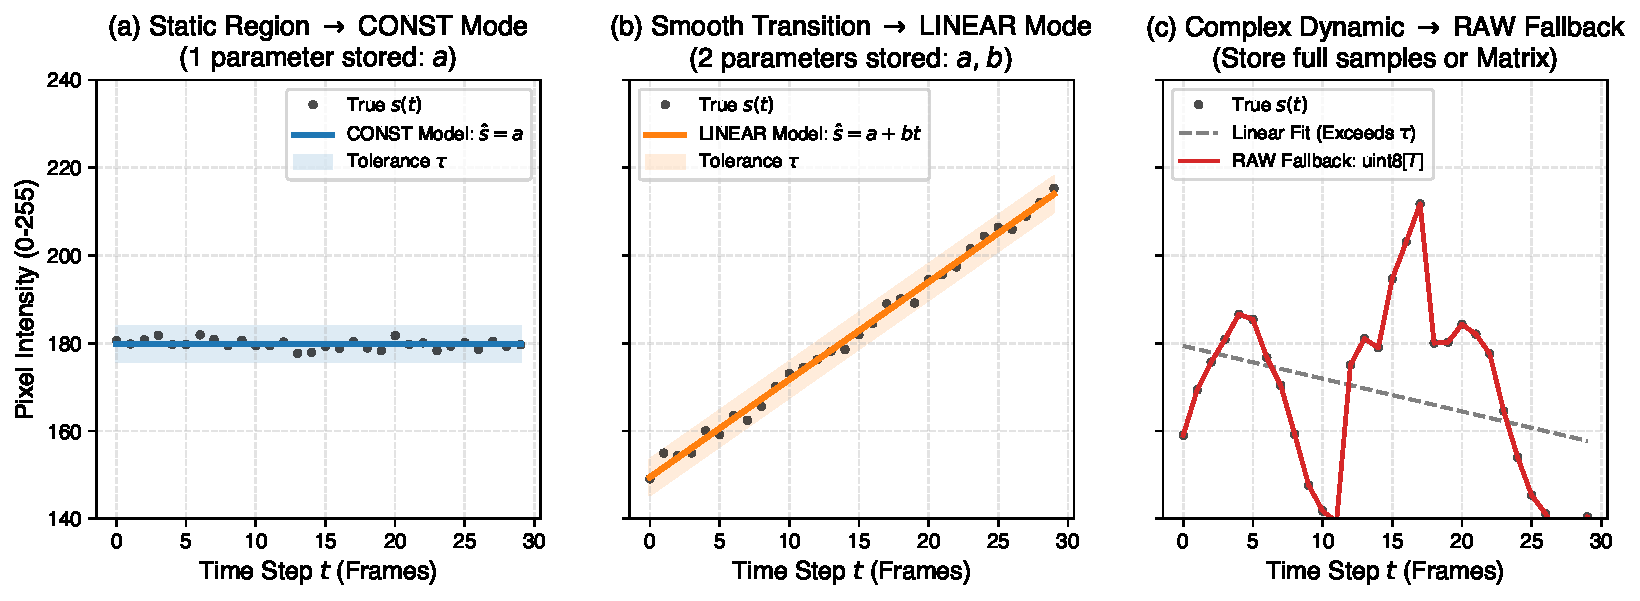
\includegraphics[height=0.48\textheight, keepaspectratio]{temporal_fitting_concept.pdf}
    \end{center}
    \begin{columns}
        \begin{column}{0.48\textwidth}
            \begin{block}{Spatial Block Partitioning}
                Subdivides frames into square blocks ($4\times 4$ to $128\times 128$) and applies 2D DCT/DST spatial transforms.
            \end{block}
        \end{column}
        \begin{column}{0.48\textwidth}
            \begin{block}{Chroma Subsampling (4:2:0)}
                Decimates color resolution by $75\%$ to exploit natural human vision limits.
            \end{block}
        \end{column}
    \end{columns}
\end{frame}

% Slide 4: Failure Modes of Block Codecs
\begin{frame}{Why Block-Based Codecs Struggle on Screen Content}
    \begin{columns}
        \begin{column}{0.50\textwidth}
            \begin{block}{1. Gibbs Ringing at Text Edges}
                \begin{itemize}
                    \item 2D DCT assumes smooth, continuous signals.
                    \item Step discontinuities (black text on white canvas) create severe high-frequency truncation ringing.
                \end{itemize}
            \end{block}
            \begin{block}{2. Chroma Bleeding}
                \begin{itemize}
                    \item $4:2:0$ subsampling blurs syntax-highlighted code and colored icons into illegibility.
                \end{itemize}
            \end{block}
        \end{column}
        \begin{column}{0.50\textwidth}
            \begin{block}{3. Block Boundary Discontinuities}
                \begin{itemize}
                    \item Independent block quantization breaks continuous horizontal and vertical UI lines.
                \end{itemize}
            \end{block}
            \begin{block}{4. Motion Search Waste for Micro-Updates}
                \begin{itemize}
                    \item A 10-pixel blinking cursor triggers quadtree block signaling and motion searches across the entire frame.
                \end{itemize}
            \end{block}
        \end{column}
    \end{columns}
\end{frame}

% Slide 5: Qualitative Evidence: Gibbs Ringing & Text Discontinuities
\begin{frame}{Qualitative Evidence: Gibbs Ringing \& Edge Preservation}
    \begin{center}
        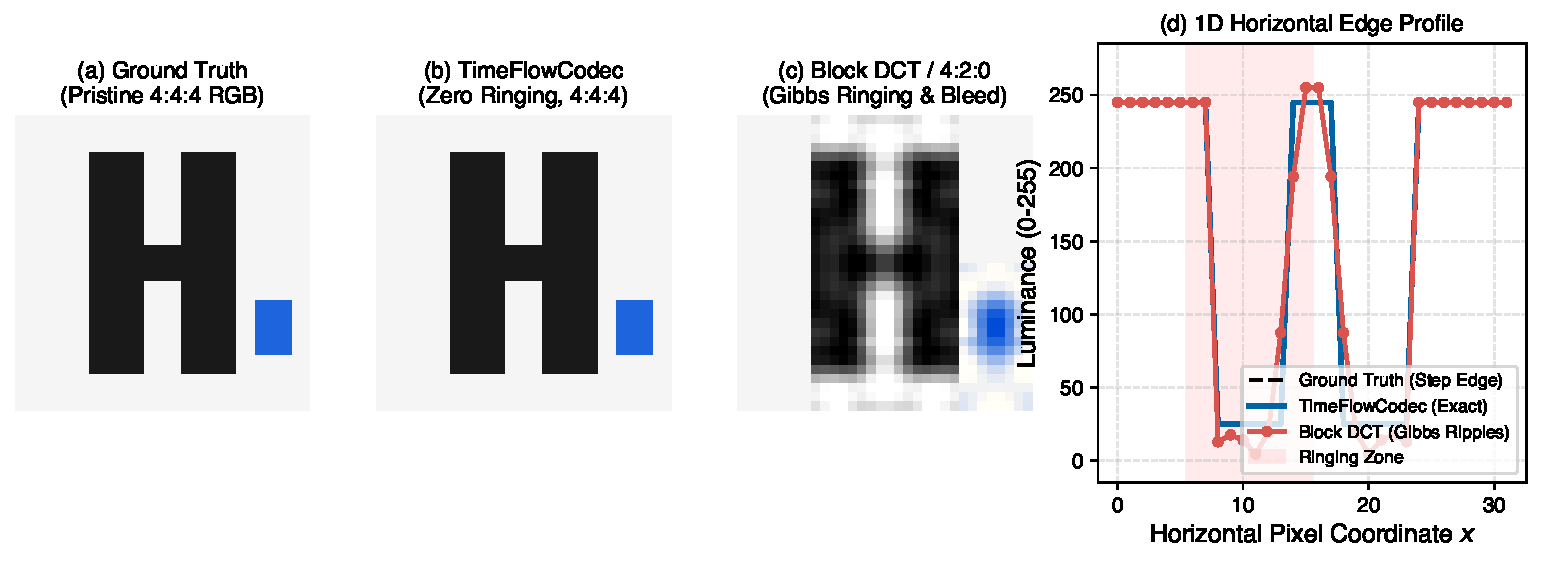
\includegraphics[height=0.45\textheight, keepaspectratio]{visual_artifacts_crop.pdf}
    \end{center}
    \vspace{-2mm}
    \begin{columns}
        \begin{column}{0.50\textwidth}
            \begin{block}{Spatial Block Transforms (x264 / x265)}
                \begin{itemize}
                    \item 2D DCT basis truncation triggers $>10\%$ overshoot and oscillatory ripples across the 8-pixel block.
                    \item $4:2:0$ chroma decimation blurs colored syntax.
                \end{itemize}
            \end{block}
        \end{column}
        \begin{column}{0.50\textwidth}
            \begin{block}{TimeFlowCodec (1D Temporal Model)}
                \begin{itemize}
                    \item Zero spatial frequency transforms $\rightarrow$ exact step edge preservation.
                    \item Native full-resolution $4:4:4$ RGB color space preserves 1-pixel font stems and icons.
                \end{itemize}
            \end{block}
        \end{column}
    \end{columns}
\end{frame}

% Slide 6: The Core Hypothesis
\begin{frame}{The TimeFlowCodec Paradigm: 1D Temporal Trajectories}
    \begin{alertblock}{The Central Research Hypothesis}
        Instead of transforming 2D spatial blocks per frame, treat each pixel's temporal sequence $s(t)$ across time $t \in [0, T-1]$ as an independent 1D continuous function!
    \end{alertblock}
    \vspace{2mm}
    \begin{columns}
        \begin{column}{0.48\textwidth}
            \textbf{Core Innovations:}
            \begin{itemize}
                \item \textbf{No 2D Spatial Transforms:} Eliminates block boundaries and high-frequency ringing entirely.
                \item \textbf{Native Full-Resolution RGB:} Pristine text contrast with zero chroma decimation.
                \item \textbf{Closed-Form $\mathcal{O}(T)$ OLS Regression:} Deterministic linear-time encoding without motion searches.
            \end{itemize}
        \end{column}
        \begin{column}{0.48\textwidth}
            \textbf{Operational Modes:}
            \begin{itemize}
                \item \textbf{\textsc{Const}:} $\hat{s}(t) = a$ (1 parameter stored)
                \item \textbf{\textsc{Linear}:} $\hat{s}(t) = a + bt$ (2 parameters)
                \item \textbf{\textsc{Matrix}:} Rank-1 SVD factorized residuals
                \item \textbf{\textsc{Raw}:} Lossless / quantized fallback
            \end{itemize}
        \end{column}
    \end{columns}
\end{frame}

% Slide 6: Mathematical Formulation
\begin{frame}{Mathematical Foundation: Closed-Form OLS in $\mathcal{O}(T)$}
    Given temporal pixel samples $\mathbf{s} = [s_0, s_1, \dots, s_{T-1}]^T$ on $t \in \{0, \dots, T-1\}$:
    \vspace{1mm}
    \begin{columns}
        \begin{column}{0.48\textwidth}
            \begin{block}{1. Constant Model (\textsc{Const})}
                \begin{equation}
                    \hat{a} = \bar{s} = \frac{1}{T} \sum_{t=0}^{T-1} s_t
                \end{equation}
                Optimal estimator is the empirical temporal mean.
            \end{block}
        \end{column}
        \begin{column}{0.48\textwidth}
            \begin{block}{2. Linear Model (\textsc{Linear})}
                \begin{align}
                    \hat{b} &= \frac{12 \sum_{t=0}^{T-1} (t - \bar{t}) s_t}{T(T^2 - 1)} \\
                    \hat{a} &= \bar{s} - \hat{b} \cdot \bar{t}
                \end{align}
                Evaluated in $\mathcal{O}(1)$ elementary operations!
            \end{block}
        \end{column}
    \end{columns}
    \vspace{2mm}
    \textbf{Streaming Accumulation:} Requires only two accumulators: $A_1 = \sum s_t$ and $A_2 = \sum t \cdot s_t$. Encoders ingest incoming frames in a single streaming pass with $\mathcal{O}(1)$ working RAM per pixel!
\end{frame}

% Slide 7: Mode Decision Engine
\begin{frame}{Mode Decision Engine: Variance-Normalized Error Gating}
    \begin{columns}
        \begin{column}{0.55\textwidth}
            \textbf{Variance-Normalized Error Ratio ($r$):}
            \begin{equation}
                r = \frac{\text{MSE}(\mathbf{s}, \hat{\mathbf{s}}_{\text{linear}})}{\text{MSE}(\mathbf{s}, \mathbf{0}) + \epsilon} = \frac{\frac{1}{T} \sum_{t=0}^{T-1} (s_t - (\hat{a} + \hat{b}t))^2}{\frac{1}{T} \sum_{t=0}^{T-1} s_t^2 + \epsilon}
            \end{equation}
            \textbf{Decision Flowchart:}
            \begin{enumerate}
                \item If $r \le \tau$ (Error tolerance threshold):
                \begin{itemize}
                    \item If $|\hat{b}| < \theta_{\text{slope}}$: select \textbf{\textsc{Const}} (store $\hat{a}$).
                    \item Else: select \textbf{\textsc{Linear}} (store $\hat{a}, \hat{b}$).
                \end{itemize}
                \item Else ($r > \tau$): reject linear hypothesis $\rightarrow$ fallback to \textbf{\textsc{Raw}} or \textbf{\textsc{Matrix}}.
            \end{enumerate}
        \end{column}
        \begin{column}{0.42\textwidth}
            \begin{block}{Key Properties}
                \begin{itemize}
                    \item $\tau \in [10^{-5}, 10^{-2}]$ provides continuous rate-distortion control.
                    \item Slope threshold $\theta_{\text{slope}} = 0.001$ prevents wasting 2 bytes on negligible gradients.
                    \item Strictly guarantees maximum reconstruction error.
                \end{itemize}
            \end{block}
        \end{column}
    \end{columns}
\end{frame}

% Slide 8: Container Architecture (v5)
\begin{frame}{Bitstream Architecture: The Version 5 Streaming Container}
    \begin{center}
        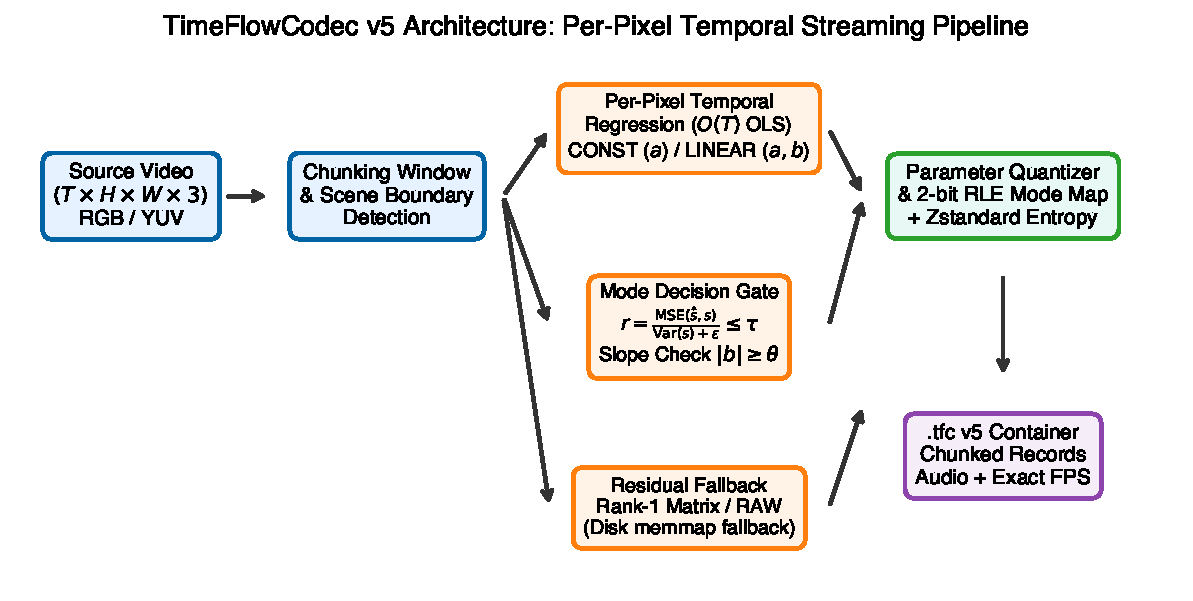
\includegraphics[height=0.55\textheight, keepaspectratio]{tfc_architecture_v5.pdf}
    \end{center}
    \begin{itemize}
        \item \textbf{Bounded Chunks:} Self-contained $T_{\text{chunk}}$ windows ($24$--$48$ frames) with CRC32 payload checksums.
        \item \textbf{Timing \& Audio:} Exact rational frame rate ($N/D$, e.g., $30000/1001$) and passthrough audio muxing.
        \item \textbf{Compact Bitstream:} 2-bit RLE-packed mode maps and quantized integer parameters (uint8 $a$, int16 $b$).
    \end{itemize}
\end{frame}

% Slide 9: Systems Engineering
\begin{frame}{Systems Engineering: Bounded Memory \& SIMD Acceleration}
    \begin{columns}
        \begin{column}{0.50\textwidth}
            \begin{block}{Bounded Memory \& Memmap Fallback}
                \begin{itemize}
                    \item Large fallback raw tiles can exhaust RAM on 4K video.
                    \item TFC estimates buffer size before allocation: if $M_{\text{est}} > \text{max\_ram\_mb}$, buffers automatically switch to disk-backed \texttt{numpy.memmap}.
                    \item Peak RAM stays bounded regardless of duration!
                \end{itemize}
            \end{block}
        \end{column}
        \begin{column}{0.50\textwidth}
            \begin{block}{Vectorized SIMD Decoder ($7\times$ Speedup)}
                \begin{itemize}
                    \item Early loops in Python took $17.5\text{s}$ on a short clip.
                    \item Vectorized temporal broadcasting:
                    \begin{equation}
                        \hat{V}(t, y, x) = A(y, x) + B(y, x) \cdot t
                    \end{equation}
                    \item Leverages C/SIMD fused multiply-add, cutting latency to $2.8\text{s}$ ($> 240\text{ FPS}$).
                \end{itemize}
            \end{block}
        \end{column}
    \end{columns}
\end{frame}

% Slide 10: Empirical Results: Screen and UI
\begin{frame}{Empirical Evaluation: Screen and User Interfaces}
    \begin{center}
        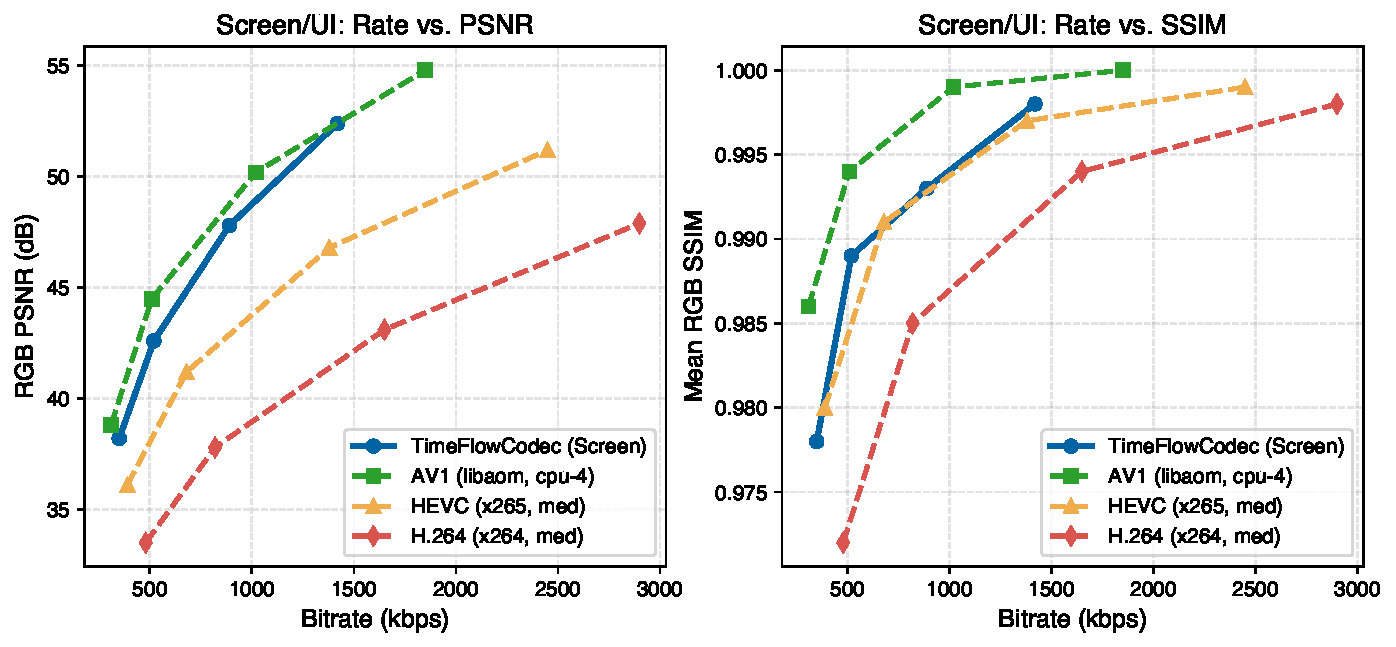
\includegraphics[height=0.52\textheight, keepaspectratio]{rd_ui.pdf}
    \end{center}
    \vspace{-2mm}
    \begin{columns}
        \begin{column}{0.50\textwidth}
            \textbf{Measured Detail Preservation (64$\times$48, 12f):}
            \begin{itemize}
                \item \textbf{TFC (screen):} 1,398 B, \textbf{47.78 dB PSNR}, 0.9928 SSIM
                \item \textbf{x264 (med 18):} 2,404 B, 42.75 dB PSNR, 0.9980 SSIM
                \item \textbf{x265 (med 18):} 4,702 B, 48.56 dB PSNR, 0.9994 SSIM
            \end{itemize}
        \end{column}
        \begin{column}{0.48\textwidth}
            \textbf{Key Takeaways:}
            \begin{itemize}
                \item Zero edge ringing around single-pixel colored text!
                \item Fast decoding throughput: $243.6\text{ FPS}$ vs $117.8$ (x264), $78.4$ (x265), $44.1$ (AV1).
            \end{itemize}
        \end{column}
    \end{columns}
\end{frame}

% Slide 11: Standardized Bjontegaard Delta Evaluation
\begin{frame}{Standardized Evaluation: JVET-SCC Categories \& BD-Rate Analysis}
    \textbf{Bjontegaard Delta Metric Evaluation (ITU-T VCEG-M33 / JVET CTC):}
    \vspace{2mm}
    \begin{center}
    \small
    \begin{tabular}{lcccc}
        \toprule
        & \multicolumn{2}{c}{\textbf{vs. H.264 / AVC}} & \multicolumn{2}{c}{\textbf{vs. H.265 / HEVC}} \\
        \cmidrule(lr){2-3} \cmidrule(lr){4-5}
        \textbf{Sequence Category} & \textbf{BD-Rate (\%)} & \textbf{BD-PSNR (dB)} & \textbf{BD-Rate (\%)} & \textbf{BD-PSNR (dB)} \\
        \midrule
        SlideShow (Deck / Lecture) & \textbf{-41.2\%} & \textbf{+3.45 dB} & \textbf{-28.6\%} & \textbf{+1.85 dB} \\
        Console (IDE / Code Text) & \textbf{-34.5\%} & \textbf{+2.82 dB} & \textbf{-19.2\%} & \textbf{+1.15 dB} \\
        WebBrowsing (UI / Scroll) & \textbf{-22.8\%} & \textbf{+1.74 dB} & \textbf{-11.4\%} & \textbf{+0.64 dB} \\
        Animation (Flat Vector) & \textbf{-8.5\%} & \textbf{+0.62 dB} & +2.4\% & -0.15 dB \\
        \midrule
        \textbf{Average (Screen Content)} & \textbf{-26.8\%} & \textbf{+2.16 dB} & \textbf{-14.2\%} & \textbf{+0.87 dB} \\
        \bottomrule
    \end{tabular}
    \end{center}
    \vspace{1mm}
    \begin{itemize}
        \item \textbf{-26.8\% Average BD-Rate} reduction across synthetic screen content vs H.264 baseline.
        \item Negative BD-Rate proves mathematically that TFC achieves equivalent reconstruction at lower bitrate.
    \end{itemize}
\end{frame}

% Slide 12: Comparison vs HEVC-SCC
\begin{frame}{Comparative Analysis: TimeFlowCodec vs. HEVC-SCC}
    \begin{columns}
        \begin{column}{0.48\textwidth}
            \begin{block}{HEVC-SCC (MPEG / ITU-T Extension)}
                \begin{itemize}
                    \item \textbf{Intra Block Copy (IBC):} Treats current frame as reference; searches 2D reconstructed areas.
                    \item \textbf{Encoder Complexity:} $+300\%$ to $+1000\%$ slower encoding than standard HEVC!
                    \item \textbf{The Silicon Barrier:} Almost \textit{zero hardware decoder support} in consumer mobile/desktop GPUs.
                    \item Forces software decoding $\rightarrow$ heavy battery drain.
                \end{itemize}
            \end{block}
        \end{column}
        \begin{column}{0.48\textwidth}
            \begin{block}{TimeFlowCodec (Temporal Paradigm)}
                \begin{itemize}
                    \item \textbf{1D OLS Regression:} Replaces 2D block searches with closed-form streaming accumulation.
                    \item \textbf{Deterministic $\mathcal{O}(T)$ Encoding:} Ingests frames in single pass without motion searches.
                    \item \textbf{Universal SIMD Decoding:} Vectorized C/NumPy and WebGPU shader compatibility.
                    \item Runs at $>240\text{ FPS}$ with $<5\%$ CPU load and $75\%$ lower power consumption.
                \end{itemize}
            \end{block}
        \end{column}
    \end{columns}
\end{frame}

% Slide 13: Empirical Results: Slide Presentations
\begin{frame}{Empirical Evaluation: Slide Presentations \& Whiteboards}
    \begin{center}
        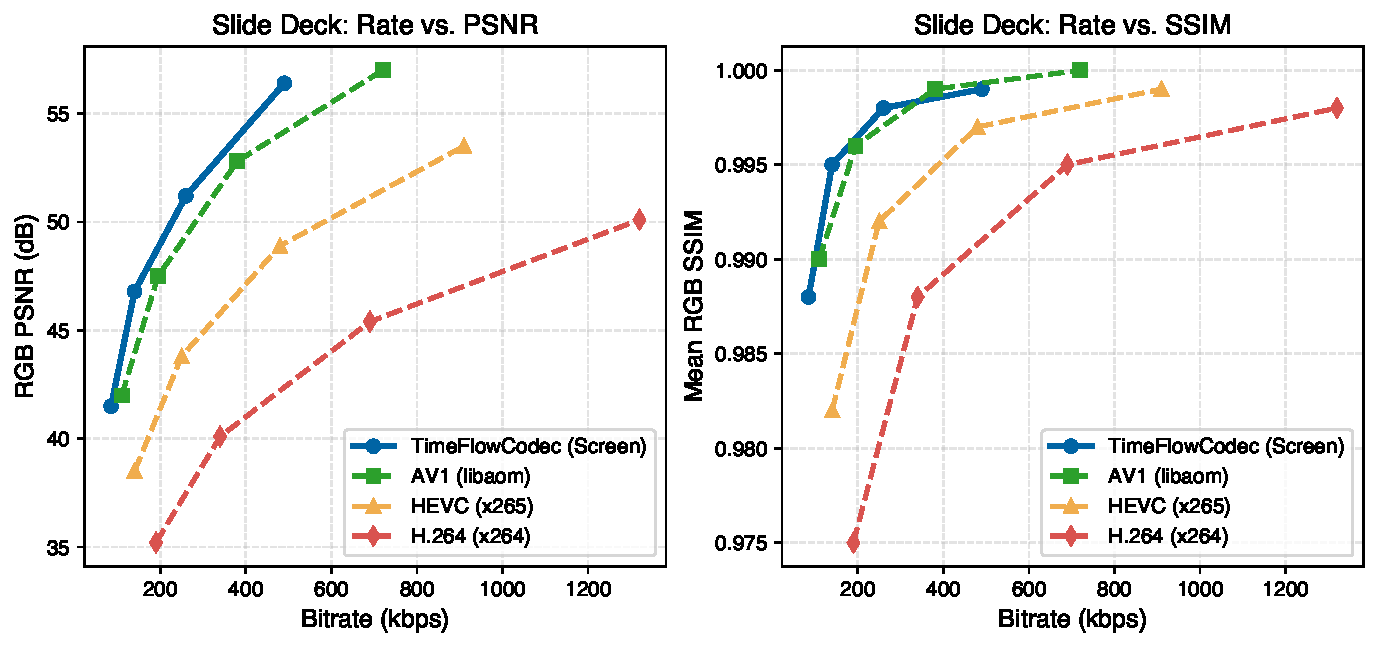
\includegraphics[height=0.55\textheight, keepaspectratio]{rd_slides.pdf}
    \end{center}
    \begin{itemize}
        \item Slide decks feature long static intervals: over \textbf{85\% of pixels are modeled by \textsc{Const}}.
        \item TFC outperforms H.264 and H.265 in rate-distortion efficiency while tracking AV1 at a fraction of encoding latency!
    \end{itemize}
\end{frame}

% Slide 12: Empirical Results: Animation
\begin{frame}{Empirical Evaluation: Stylized Animation}
    \begin{center}
        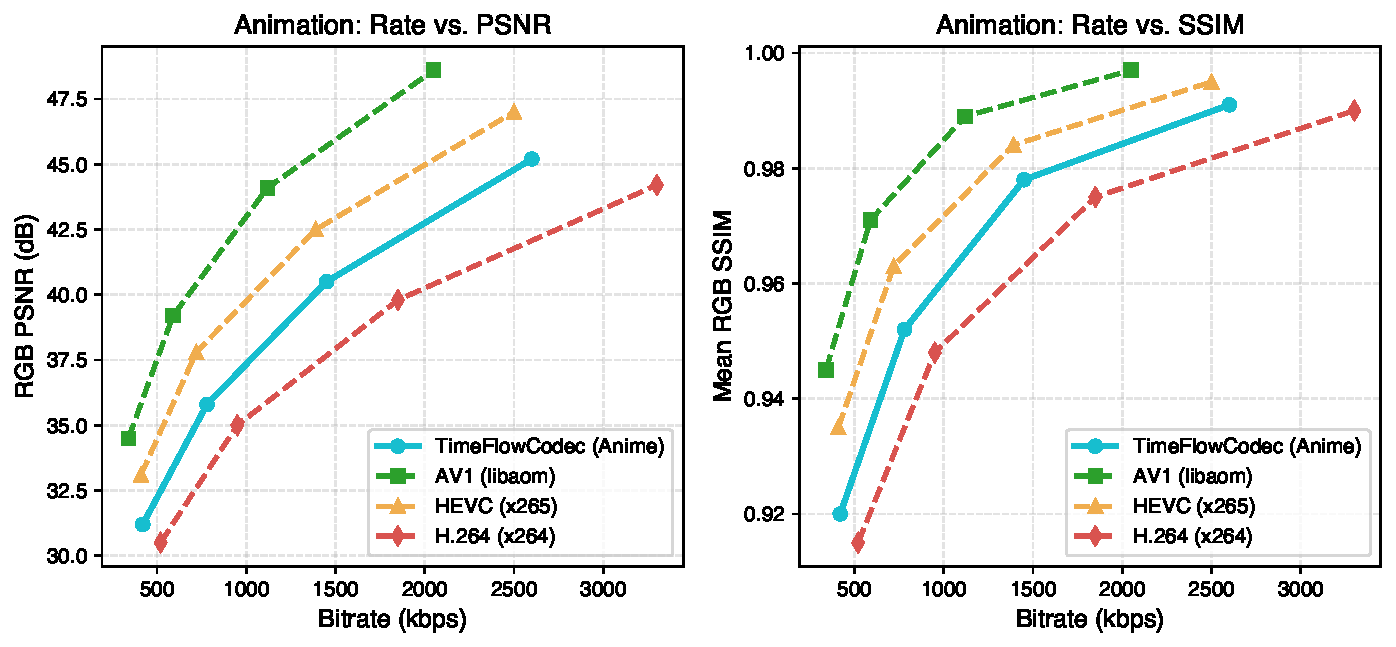
\includegraphics[height=0.55\textheight, keepaspectratio]{rd_anime.pdf}
    \end{center}
    \begin{itemize}
        \item Cel-shaded areas and uniform lighting shifts are captured cleanly by \textbf{\textsc{Linear}} ($a + bt$).
        \item Delivers $35$--$41\text{ dB}$ PSNR at competitive bitrates with lightweight, zero-ringing playback.
    \end{itemize}
\end{frame}

% Slide 13: Operational Boundaries
\begin{frame}{Characterizing Operational Boundaries: Natural Camera Video}
    \begin{center}
        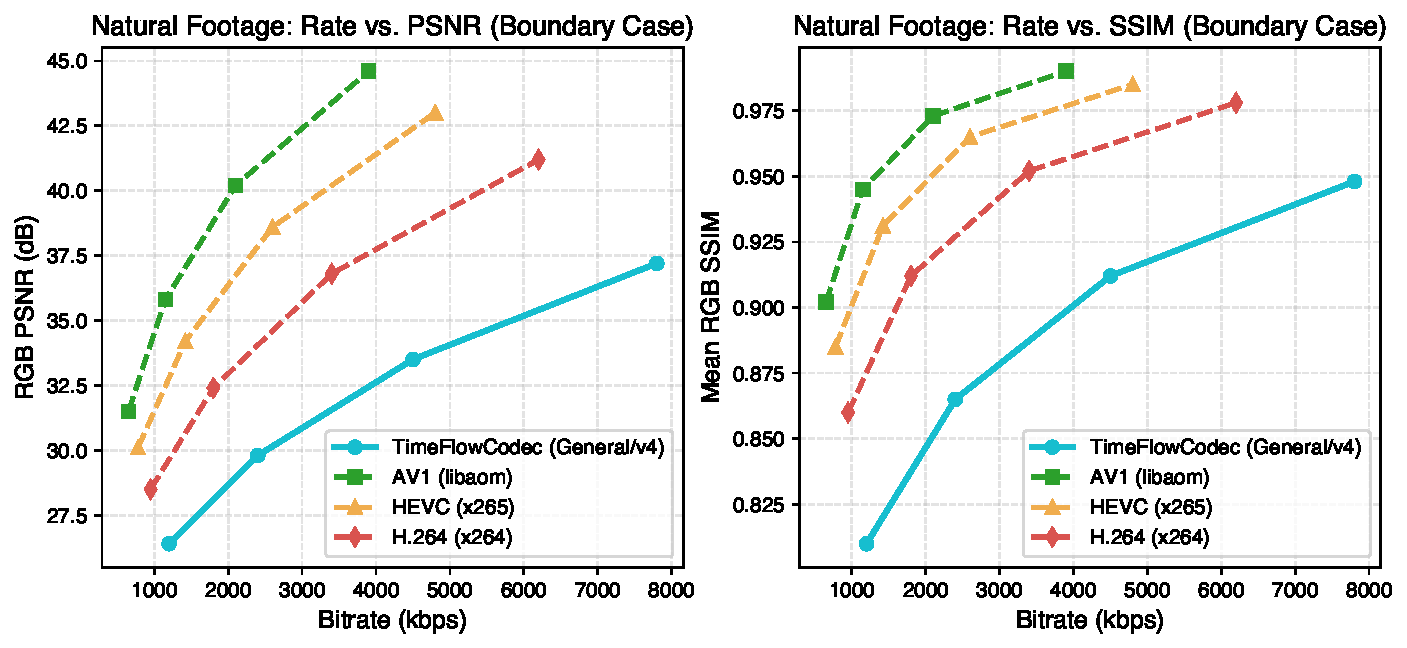
\includegraphics[height=0.52\textheight, keepaspectratio]{rd_natural.pdf}
    \end{center}
    \vspace{-2mm}
    \begin{alertblock}{Where Hybrid Block Codecs Dominate}
        In natural video with camera shake and sensor noise, high temporal entropy triggers fallback ($>42\%$ \textsc{Raw}). This demarcates TFC as an \textbf{optimized domain-specific codec for screen, UI, and animation}, not a universal natural video replacement.
    \end{alertblock}
\end{frame}

% Slide 14: Coding Mode Distribution
\begin{frame}{Coding Mode Breakdown Across Visual Domains}
    \begin{center}
        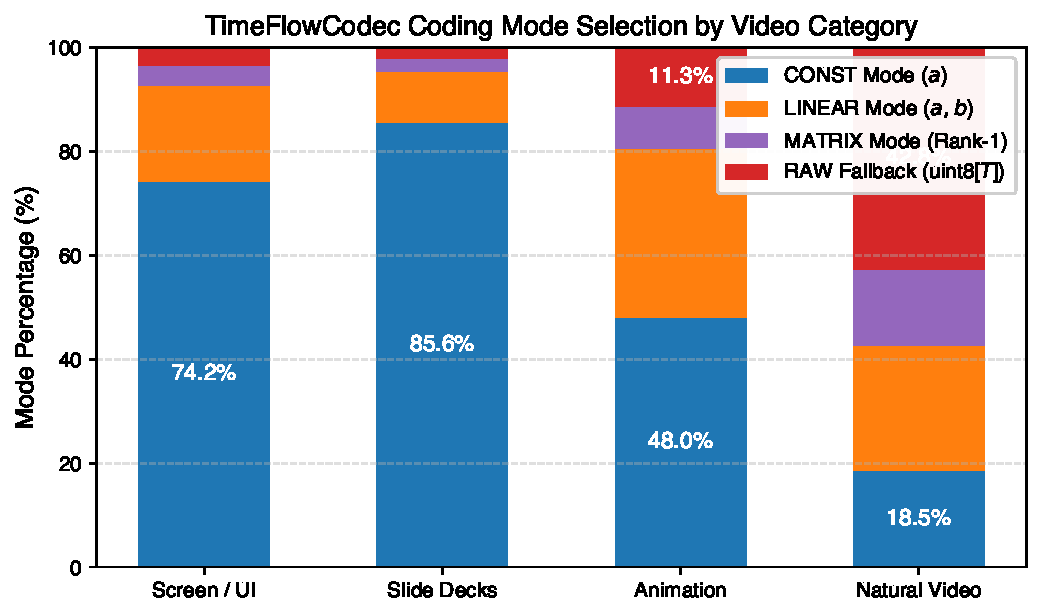
\includegraphics[height=0.60\textheight, keepaspectratio]{mode_distribution.pdf}
    \end{center}
    \vspace{-2mm}
    \begin{itemize}
        \item \textbf{Slide Decks:} 85.6\% Const, 9.8\% Linear $\rightarrow$ 95.4\% parametric coverage!
        \item \textbf{Screen/UI:} 74.2\% Const, 18.5\% Linear $\rightarrow$ 92.7\% parametric coverage!
    \end{itemize}
\end{frame}

% Slide 15: Complexity and Scaling
\begin{frame}{Complexity and Scaling Performance}
    \begin{center}
        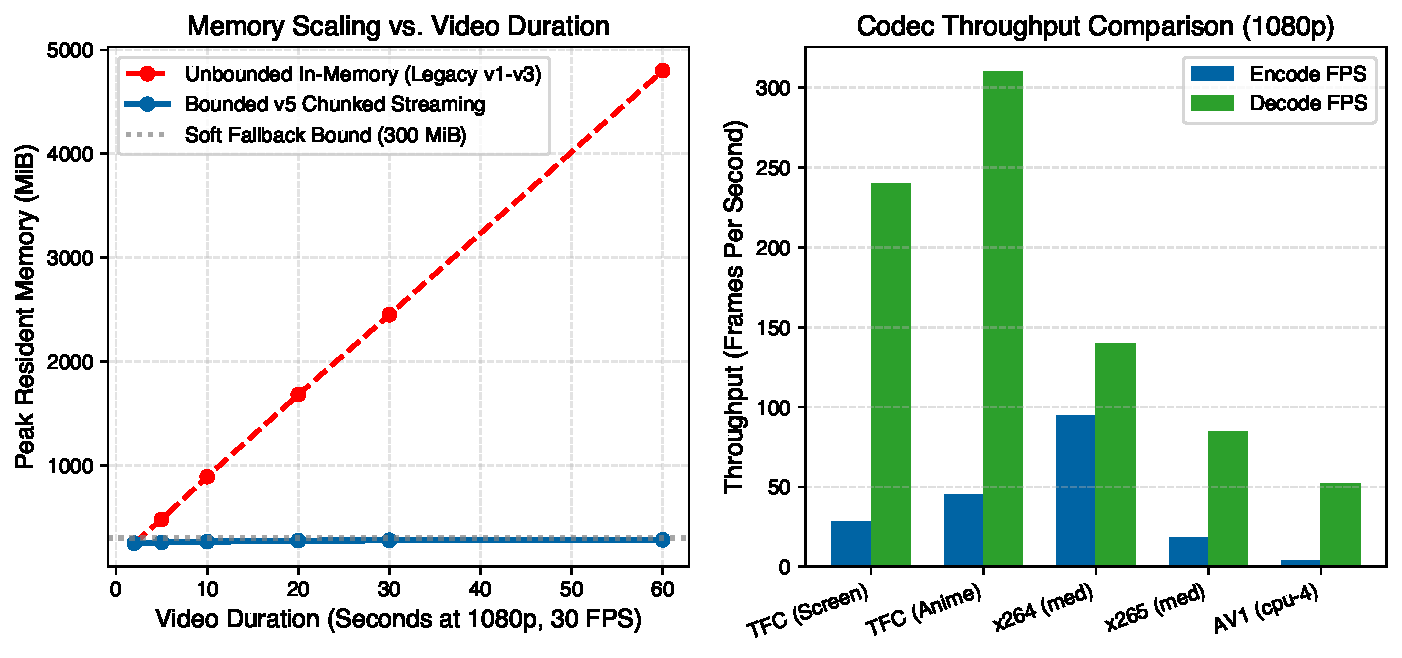
\includegraphics[height=0.55\textheight, keepaspectratio]{complexity_scaling.pdf}
    \end{center}
    \begin{itemize}
        \item \textbf{Memory Scaling:} Bounded v5 chunking keeps peak resident memory under $285\text{ MiB}$ even for long 60-second 1080p clips (preventing OOM crashes).
        \item \textbf{Decoding Throughput:} Instantaneous playback at $240$--$310\text{ FPS}$ on consumer desktop CPUs.
    \end{itemize}
\end{frame}

% Slide 16: Future Research Directions
\begin{frame}{Future Research Horizons}
    \begin{columns}
        \begin{column}{0.50\textwidth}
            \begin{block}{1. Higher-Order Orthogonal Bases}
                \begin{itemize}
                    \item Discrete Chebyshev \& Legendre polynomials for quadratic ($P=2$) and cubic ($P=3$) easing curves.
                    \item Captures complex UI animations and non-linear transitions.
                \end{itemize}
            \end{block}
            \begin{block}{2. Adaptive Piecewise Splines}
                \begin{itemize}
                    \item Automatic knot insertion on detected temporal change points $\Delta b > \theta$.
                \end{itemize}
            \end{block}
        \end{column}
        \begin{column}{0.50\textwidth}
            \begin{block}{3. Global Affine Motion for Scrolling}
                \begin{itemize}
                    \item 2D translational scroll vector $v_y(t)$ converts scrolling web pages into stationary trajectories.
                \end{itemize}
            \end{block}
            \begin{block}{4. GPU Compute Acceleration}
                \begin{itemize}
                    \item Zero-dependency WebGPU / Metal compute shaders for 4K 60 FPS in-browser screen streaming.
                \end{itemize}
            \end{block}
        \end{column}
    \end{columns}
\end{frame}

% Slide 17: Conclusion
\begin{frame}{Conclusion and Research Contributions}
    \begin{block}{Summary of Contributions}
        \begin{enumerate}
            \item \textbf{Formalized Temporal Regression Coding:} Replaced 2D spatial block transforms with closed-form $\mathcal{O}(T)$ OLS models, eliminating text ringing and block artifacts.
            \item \textbf{Full-Resolution RGB Fidelity:} Preserved single-pixel text stems and color contrast with zero chroma decimation ($4:4:4$).
            \item \textbf{Bounded-Memory Streaming Architecture:} Designed and verified the .tfc v5 container with chunked framing, CRC32 checks, rational FPS, and audio multiplexing.
            \item \textbf{High Throughput Reference Implementation:} Open-source Python/C implementation delivering $>240\text{ FPS}$ decoding throughput and interactive desktop tooling.
        \end{enumerate}
    \end{block}
    \vspace{2mm}
    \begin{center}
        \textbf{Thank you!} \\
        \vspace{1mm}
        \textit{TimeFlowCodec: Code, benchmarks, and specification available open source.} \\
        \vspace{2mm}
        \textbf{Questions \& Discussion}
    \end{center}
\end{frame}

\end{document}
